\documentclass[11pt]{article}
\usepackage{geometry, titlesec}
\usepackage[parfill]{parskip}
\usepackage[italicdiff]{physics}
\usepackage{amsfonts, amsthm}
\usepackage[cm]{fullpage}
\usepackage{fancyhdr}
\usepackage{enumitem}
\usepackage{xcolor, soul}
\usepackage{graphicx}
\usepackage{siunitx}
%\allowdisplaybreaks

\renewcommand{\thesubsection}{\thesection.\alph{subsection}}
\setenumerate[1]{label={(\alph*)}}

\makeatletter
\renewcommand*\env@cases[1][1.2]{%
  \let\@ifnextchar\new@ifnextchar
  \left\lbrace
  \def\arraystretch{#1}%
  \array{@{}l@{\quad}l@{}}%
}
\makeatother
 
\renewcommand{\footrulewidth}{.2pt}
%\setlist[enumerate]{leftmargin=*}
\pagestyle{fancy}
\fancyhf{}
\lhead{Physics 131-B}
\chead{\textbf{Homework 6 Solutions}}
\rhead{Lacey Rainbolt}
\setlength{\headheight}{11pt}
\setlength{\headsep}{11pt}
\setlength{\footskip}{24pt}
\lfoot{\today}
\rfoot{\thepage}

\titleformat{\subsection}[runin]{\normalfont\large\bfseries}{\thesubsection}{1em}{}
\newcommand{\refeq}[1]{(\ref{#1})}

\newcommand{\beq}{\begin{equation*}}
\newcommand{\eeq}{\end{equation*}}

\newcommand{\beqn}{\begin{equation}}
\newcommand{\eeqn}{\end{equation}}

\newcommand{\blg}{\begin{align*}}
\newcommand{\elg}{\end{align*}}


\newenvironment{statement}
{
    \color{gray}
    \ignorespaces
}
{
%    \smallskip
}

\newenvironment{problem}
{
    \color{darkgray}
    \ignorespaces
}

\newenvironment{solution}
{
    \paragraph{Solution.}
    \ignorespaces
}
{
    \bigskip
}

\renewcommand{\vec}[1]{\mathbf{#1}}


\begin{document}

\begin{figure} \centering
	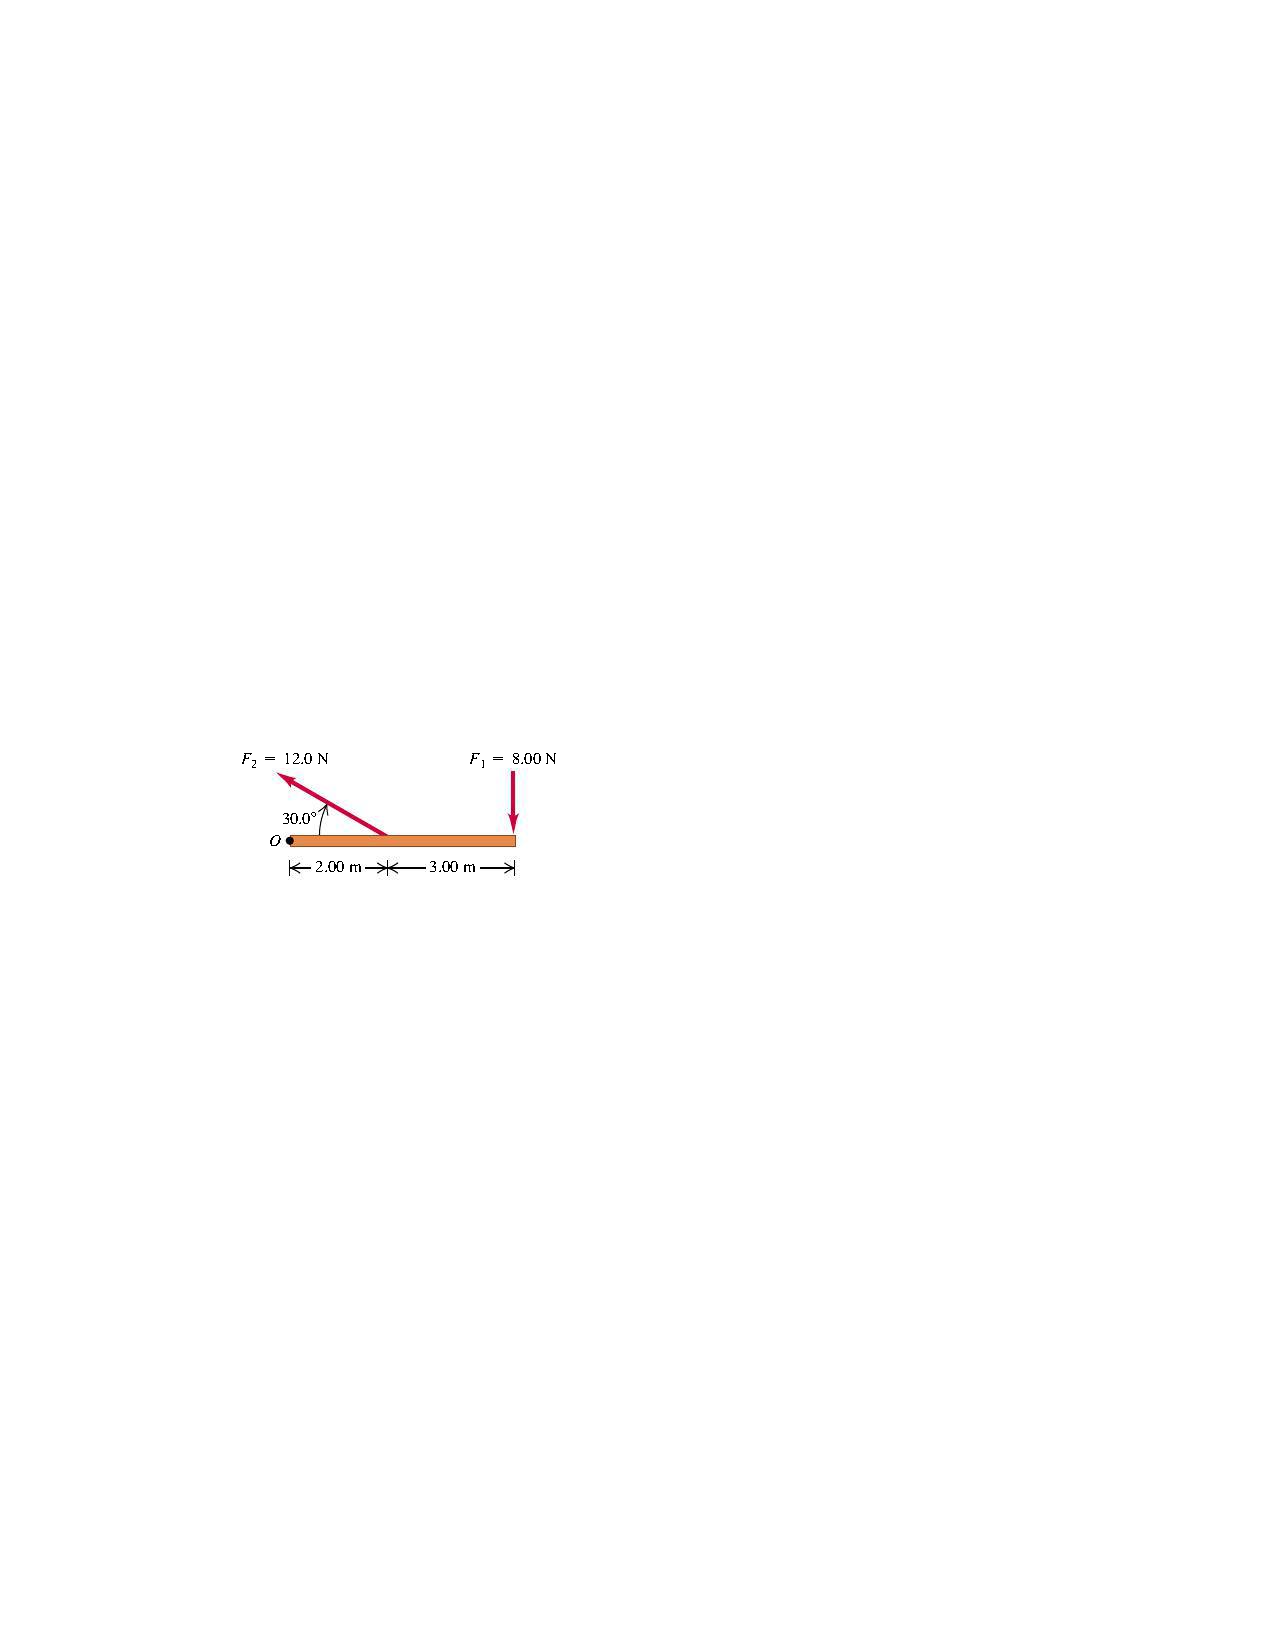
\includegraphics{E10-2}
	\caption{\textbf{E10.2}}
	\label{E10.2}
\end{figure}

\paragraph{Exercise 10.2}
\begin{problem}
	Calculate the net torque about point $O$ for the two forces applied as in Fig.~\ref{E10.2}.  The rod and both forces are in the plane of the page.
\end{problem}

%\begin{figure} \centering
	
%	\label{E10.2}
%\end{figure}

\newcommand{\ih}{\vec{\,\hat{i}}}
\newcommand{\jh}{\vec{\,\hat{j}}}
\newcommand{\kh}{\vec{\,\hat{k}}}

\newcommand{\vF}{\vec{F}}
\newcommand{\vt}{\boldsymbol{\tau}}
\newcommand{\vr}{\vec{r}}

\newcommand{\vFq}{\vF_1}
\newcommand{\Fq}{F_1}
\newcommand{\vFw}{\vF_2}
\newcommand{\Fw}{F_2}

\newcommand{\vtq}{\vt_1}
\newcommand{\vtw}{\vt_2}
\newcommand{\vrq}{\vr_1}
\newcommand{\rrq}{r_1}
\newcommand{\vrw}{\vr_2}
\newcommand{\rw}{r_2}

\newcommand{\vtnet}{\vt_\text{net}}
\newcommand{\tnet}{\tau_\text{net}}


\begin{solution}
	This problem is a simple plug and chug to help us practice calculating cross products and torques.  The net torque on the rod is the sum of the torques due to each of the forces:
	\beqn \label{nett}
		\vtnet = \vtq + \vtw.
	\eeqn
	Here, $\vtq$ is the~(vector) torque due to $\vFq$ relative to point $O$.  Let $\vrq$ be the vector from $O$ to where $\vFq$ acts on the rod.  Using the coordinate axes drawn in Fig.~\ref{E10.2}, we have
	\begin{align*}
		\vrq &= \rrq \ih, \\
		\vFq &= -\Fq \jh,
	\end{align*}
	where $\rrq = \SI{5.00}{\meter}$ and $\Fw = \SI{8.00}{\newton}$.  Then
	\beq
		\vtq = \vrq \times \vFq = -\rrq \Fq \kh.
	\eeq
	Now for $\vtw$, define $\vrw$ as the vector from $O$ to where $\vFw$ acts on the rod.  Then
		\begin{align*}
		\vrw &= \rw \ih, \\
		\vFw &= -(\Fw \cos{30.0^\circ}) \ih + (\Fw \sin{30.0^\circ}) \jh = -\frac{\sqrt{3}}{2} \Fw \ih + \frac{1}{2} \Fw \jh,
	\end{align*}
	where $\rw = \SI{2.00}{\meter}$ and $\Fw = \SI{12.0}{\newton}$, and
	\beq
		\vtw = \vrw \times \vFw = \frac{1}{2} \rw \Fw \kh.
	\eeq
	Feeding our results into \refeq{nett},
	\beq
		\vtnet = \left( \rrq \Fq - \frac{1}{2} \rw \Fw \right)\!\kh.
	\eeq
	Plugging everything in,
	\beq
		\vtnet = \left( -\rrq \Fq + \frac{1}{2} \rw \Fw \right) \kh = \left( -(\SI{5.00}{\meter}) (\SI{8.00}{\newton}) + \frac{1}{2} (\SI{2.00}{\meter}) (\SI{12.0}{\newton}) \right) \kh = -(\SI{28.0}{\newton\meter}) \kh.
	\eeq
	So the torque has magnitude $\tnet = {\color{blue} \SI{28.0}{\newton\meter}}$ and is acting {\color{blue} clockwise}.
\end{solution}

\newcommand{\mb}{m_b}
\newcommand{\mw}{m_w}
\newcommand{\mmp}{m_p}

\newcommand{\simb}{\SI{12.0}{\kg} }
\newcommand{\simw}{\SI{5.00}{\kg} }
\newcommand{\simp}{\SI{2.00}{\kg} }
\newcommand{\sIip}{\SI{0.0625}{\kg\square\meter} }

\newcommand{\sig}{\SI{9.81}{\meter\per\square\second} }

\newcommand{\Ww}{W_w}
\newcommand{\aq}{a_b}

\newcommand{\Tb}{T_b}
\newcommand{\Tw}{T_w}

\newcommand{\az}{\alpha_z}

\newcommand{\Nx}{N_x}
\newcommand{\Ny}{N_y}

\clearpage
\paragraph{Exercise 10.16}
\begin{problem}
	A \simb box resting on a horizontal, frictionless surface is attached to a \simp weight by a thin, light wire that passes over a frictionless pulley (Fig.~\ref{E10.16}).  The pulley has the shape of a uniform solid disk of mass \simp and diameter \SI{0.500}{\meter}.  After the system is released, find
	\begin{enumerate}
		\item the tension in the wire on both sides of the pulley,
		\item the acceleration of the box, and
		\item the horizontal and vertical components of the force that the axle exerts on the pulley.
	\end{enumerate}
\end{problem}

\begin{figure} \centering
	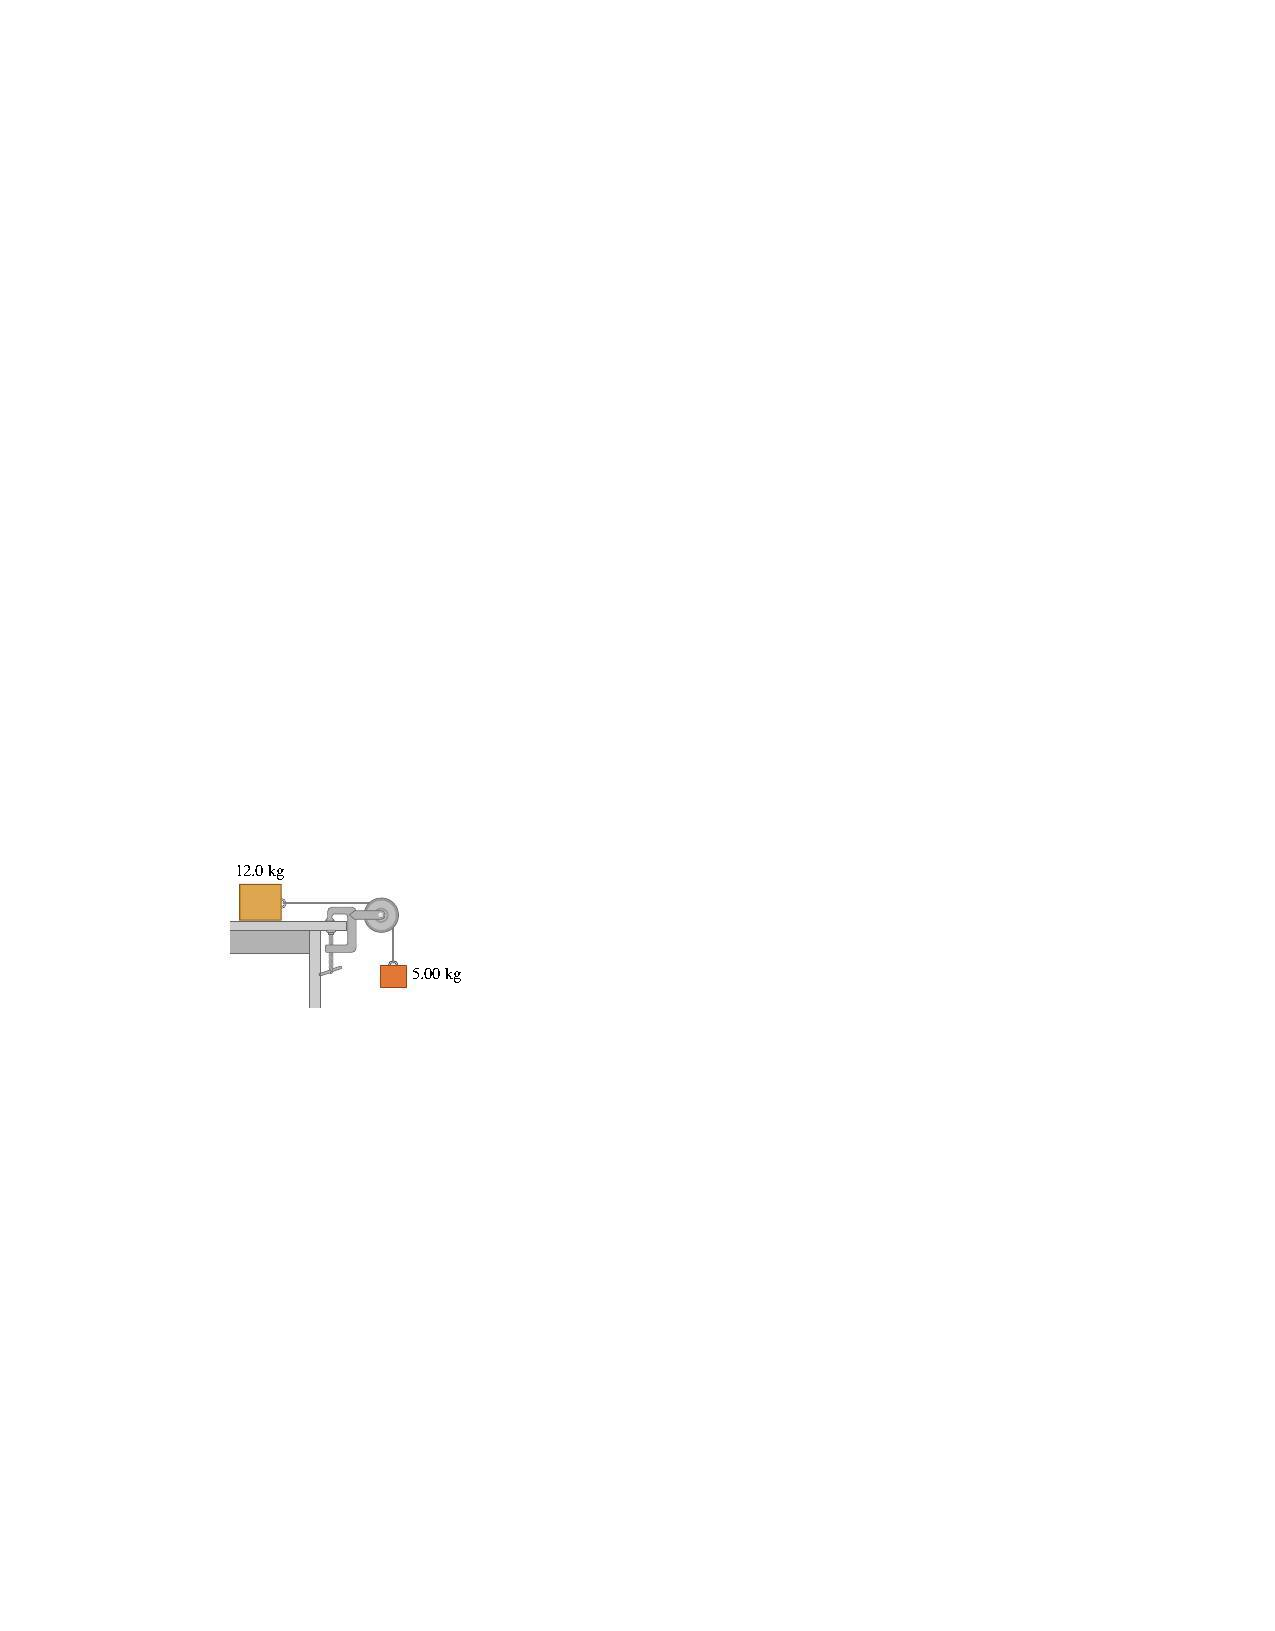
\includegraphics{E10-16}
	\caption{\textbf{E10.16}}
	\label{E10.16}
\end{figure}

\begin{figure}[b]
	\vspace{1.5in}
	\caption{Free-body diagrams for 10.16(a).}
	\label{E10.16a}
\end{figure}

\begin{solution}
	The box and the weight must have the same acceleration $a$ since they are connected by the wire.  It is safe to assume the pulley rolls without slipping against the wire (otherwise it would not be a very effective pulley!), so its tangential acceleration is also $a$.  This is the key we need to solve the problem.
	
	We can draw a free-body diagram for each object, as shown in Fig.~\ref{E10.16a}.  Using these diagrams, we can write down three equations using Newton's second law: one for the box of mass $\mb$,
	\beqn \label{box}
		\mb a = \Tb,
	\eeqn
	one for the weight of mass $\mw$,
	\beqn \label{weight}
		\mw a = \mw g - \Tw.
	\eeqn
	and one for the pulley (which we will write generally for now),
	\beqn \label{pulley0}
		\tnet = I \alpha = I \frac{a}{r}.
	\eeqn
	Here, $I$ is the moment of inertia about the pulley's center and $\alpha$ its angular acceleration.  Since the pulley rolls without slipping, $\alpha = a / r$, where $r$ is the radius of the pulley.
			
	$\Tw$ and $\Tb$ each exert a torque on the outer edge of the pulley, but in opposite directions.  We know the weight must be moving downward, meaning $\Tw$ has a greater magnitude, and so the pulley is rotating in the direction due to $\tau_w$.  The lever arm for each torque is the radius of the pulley $r$.  Putting this all together,
	\beq
		\tnet = \tau_w + \tau_b = \Tw r - \Tb r.
	\eeq
	The pulley is a solid cylinder rotating about its $z$ axis with mass $\mmp$.  Then
	\beq
		I = \frac{1}{2} \mmp r^2,
	\eeq
	and \refeq{pulley0} can be rewritten as follows:
	\beqn \label{pulley}
		(\Tw - \Tb) r = \frac{1}{2} \mmp r^2 \frac{a}{r} \implies \Tw - \Tb = \frac{1}{2} \mmp a.
	\eeqn
	Notice that if $\mmp = 0$, we would have $\Tb = \Tw$; that is, equal tension in the wire on either side of the pulley.  This is the idealized case we studied in earlier problems involving \emph{massless} pulleys.

	Getting back to the problem at hand, the system of three equations \refeq{box}, \refeq{weight}, and \refeq{pulley} has three unknowns.  The solutions are
	\begin{align}
		\Tb &= 2g \frac{\mb \mw}{2 \mb + 2 \mw + \mmp}, \label{Tb} \\
		\Tw &= g \mw \frac{2 \mb + \mmp}{2 \mb + 2 \mw + \mmp}, \label{Tw} \\
		a &= 2g \frac{\mw}{2 \mb + 2 \mw + \mmp}. \label{acc}
	\end{align}
			
	\begin{enumerate}
		\item Plugging numbers into \refeq{Tb} and \refeq{Tw} gives us
			\begin{align*}
				\Tb &= 2 (\sig) \frac{(\simb) (\simw)}{2 (\simb) + 2 (\simw) + (\simp)} = {\color{blue} \SI{32.7}{\newton}}, \\
				\Tw &= (\sig) (\simw) \frac{2 (\simb) + (\simp)}{2 (\simb) + 2 (\simw) + (\simp)} = {\color{blue} \SI{35.4}{\newton}}.
			\end{align*}
		
		\item Plugging numbers into \refeq{acc} gives us
			\beq
				a = 2 (\sig) \frac{(\simw)}{2 (\simb) + 2 (\simw) + (\simp)} = {\color{blue} \SI{2.73}{\meter\per\square\second}}.
			\eeq
			
		\item The pulley is not moving up or down.  This means the axle must be exerting a normal force $\vec{N}$ upon its center of mass which exactly cancels all other forces acting upon it.  The relevant free-body diagram is shown in Fig.~\ref{E10.16c}.  Balancing forces in the vertical direction, we have
		\beq
			\Ny = \Tw + \mmp g = \SI{35.4}{\newton} + (\simp) (\sig) = {\color{blue} \SI{55.0}{\newton}},
		\eeq
		and in the horizontal direction,
		\beq
			\Nx = \Tb = {\color{blue} \SI{32.7}{\newton}}.
		\eeq
	\end{enumerate}
\end{solution}

\begin{figure}[b]
	\caption{Free-body diagram for 10.16(c).}
	\label{E10.16c}
\end{figure}


\clearpage
\begin{figure} \centering
	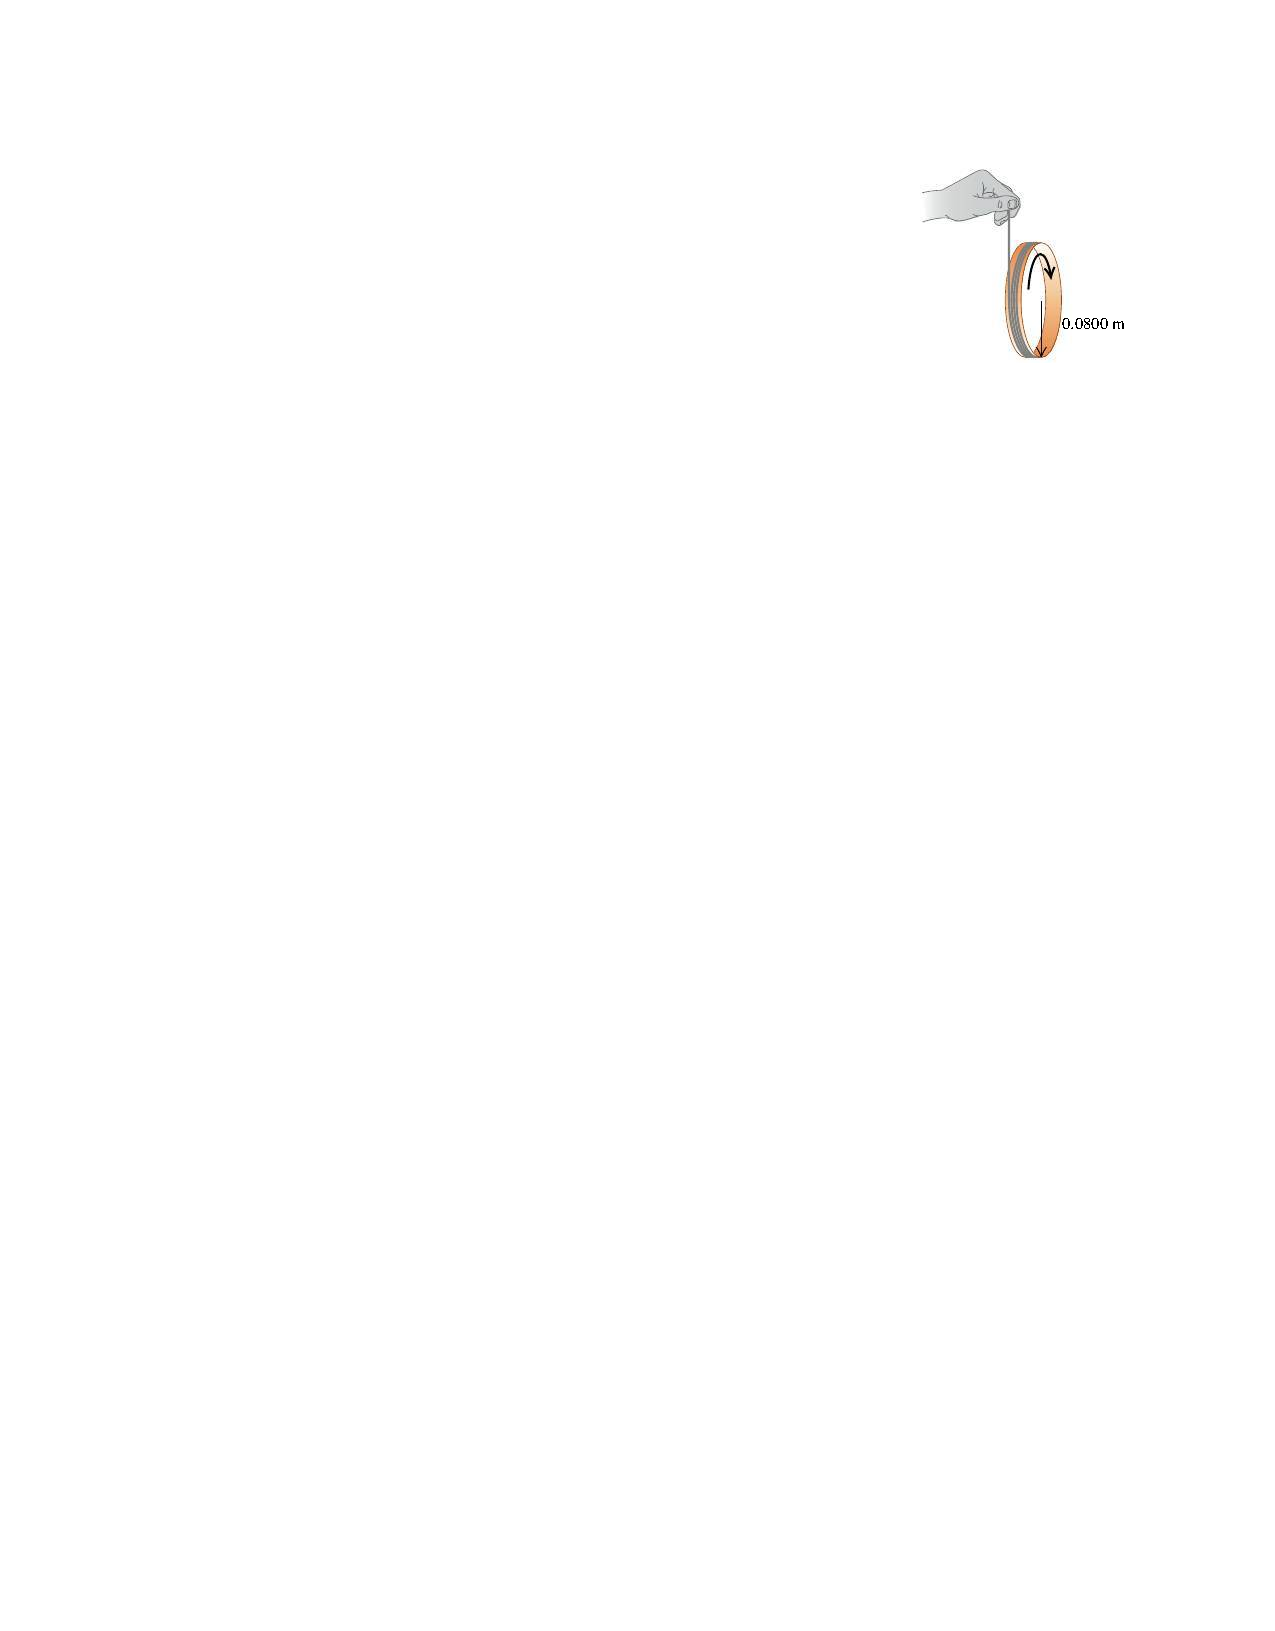
\includegraphics{E10-22}
	\caption{\textbf{E10.22}}
	\label{E10.22}
\end{figure}

\newcommand{\Ug}{U_g}

\paragraph{Exercise 10.22}
\begin{problem}
	A string is wrapped several times around the rim of a small hoop with radius \SI{8.00}{\centi\meter} and mass \SI{0.180}{\kilo\gram}.  The free end of the string is held in place and the hoop is released from rest (Fig.~\ref{E10.22}).  After the hoop has descended \SI{75.0}{\centi\meter}, calculate
	\begin{enumerate}
		\item the angular speed of the rotating hoop, and
		\item the speed of its center.
	\end{enumerate}
\end{problem}

\begin{solution}
	We can solve this problem using conservation of energy.  The ring starts from rest and then experiences both translational and rotational motion.  In the initial and final states of the system, respectively, the hoop's kinetic energy is given by
	\begin{align*}
		K_i &= 0, &
		K_f &= \frac{1}{2} m v^2 + \frac{1}{2} I \omega^2,
	\end{align*}
	where $v$ is the (translational) speed of its center, $I$ the moment of inertia about its center of mass, and $\omega$ is its angular speed.  For a hoop,
	\beq
		I = m r^2.
	\eeq
	Once the hoop has descended $h = \SI{75.0}{\centi\meter}$, its gravitational potential energy has decreased.  This is the only source of potential energy for the hoop.  We will fix our zero point at \SI{75.0}{\cm} below the hoop, so
	\begin{align*}
		U_i &= mg h, &
		U_f &= 0.
	\end{align*}
	Invoking conservation of energy,
	\beqn \label{conse}
		\Delta K + \Delta U = 0 \implies mg h = \frac{1}{2} m v^2 + \frac{1}{2} m r^2 \omega^2.
	\eeqn
	We need to invoke another condition in order to solve for the \emph{two} unknowns $v$ and $\omega$.  Once again, this is rolling without slipping: the edge of the hoop must be moving at the same speed that the string is unwinding.  This means
	\beqn \label{roll}
		v = r \omega,
	\eeqn
	which we can substitute into \refeq{conse} to obtain
	\beqn \label{conse2}
		m g h = \frac{1}{2} m r^2 \omega^2 + \frac{1}{2} m r^2 \omega^2 \implies g \,h = r^2 \omega^2.
	\eeqn
	
	\begin{enumerate}
		\item Rearranging \refeq{conse2} and plugging in numbers,
			\beq
				\omega = \frac{\sqrt{g h}}{r} = \frac{\sqrt{(\sig) (\SI{0.750}{\meter})}}{\SI{8.00e-2}{\meter}} = {\color{blue} \SI{33.9}{\radian\per\second}}.
			\eeq
			
		\item Now plugging into \refeq{roll},
			\beq
				v = (\SI{8.00e-2}{\meter}) (\SI{33.9}{\radian\per\second}) = {\color{blue} \SI{2.71}{\meter\per\second}}.
			\eeq
	\end{enumerate}
\end{solution}

\clearpage
\begin{figure} \centering
	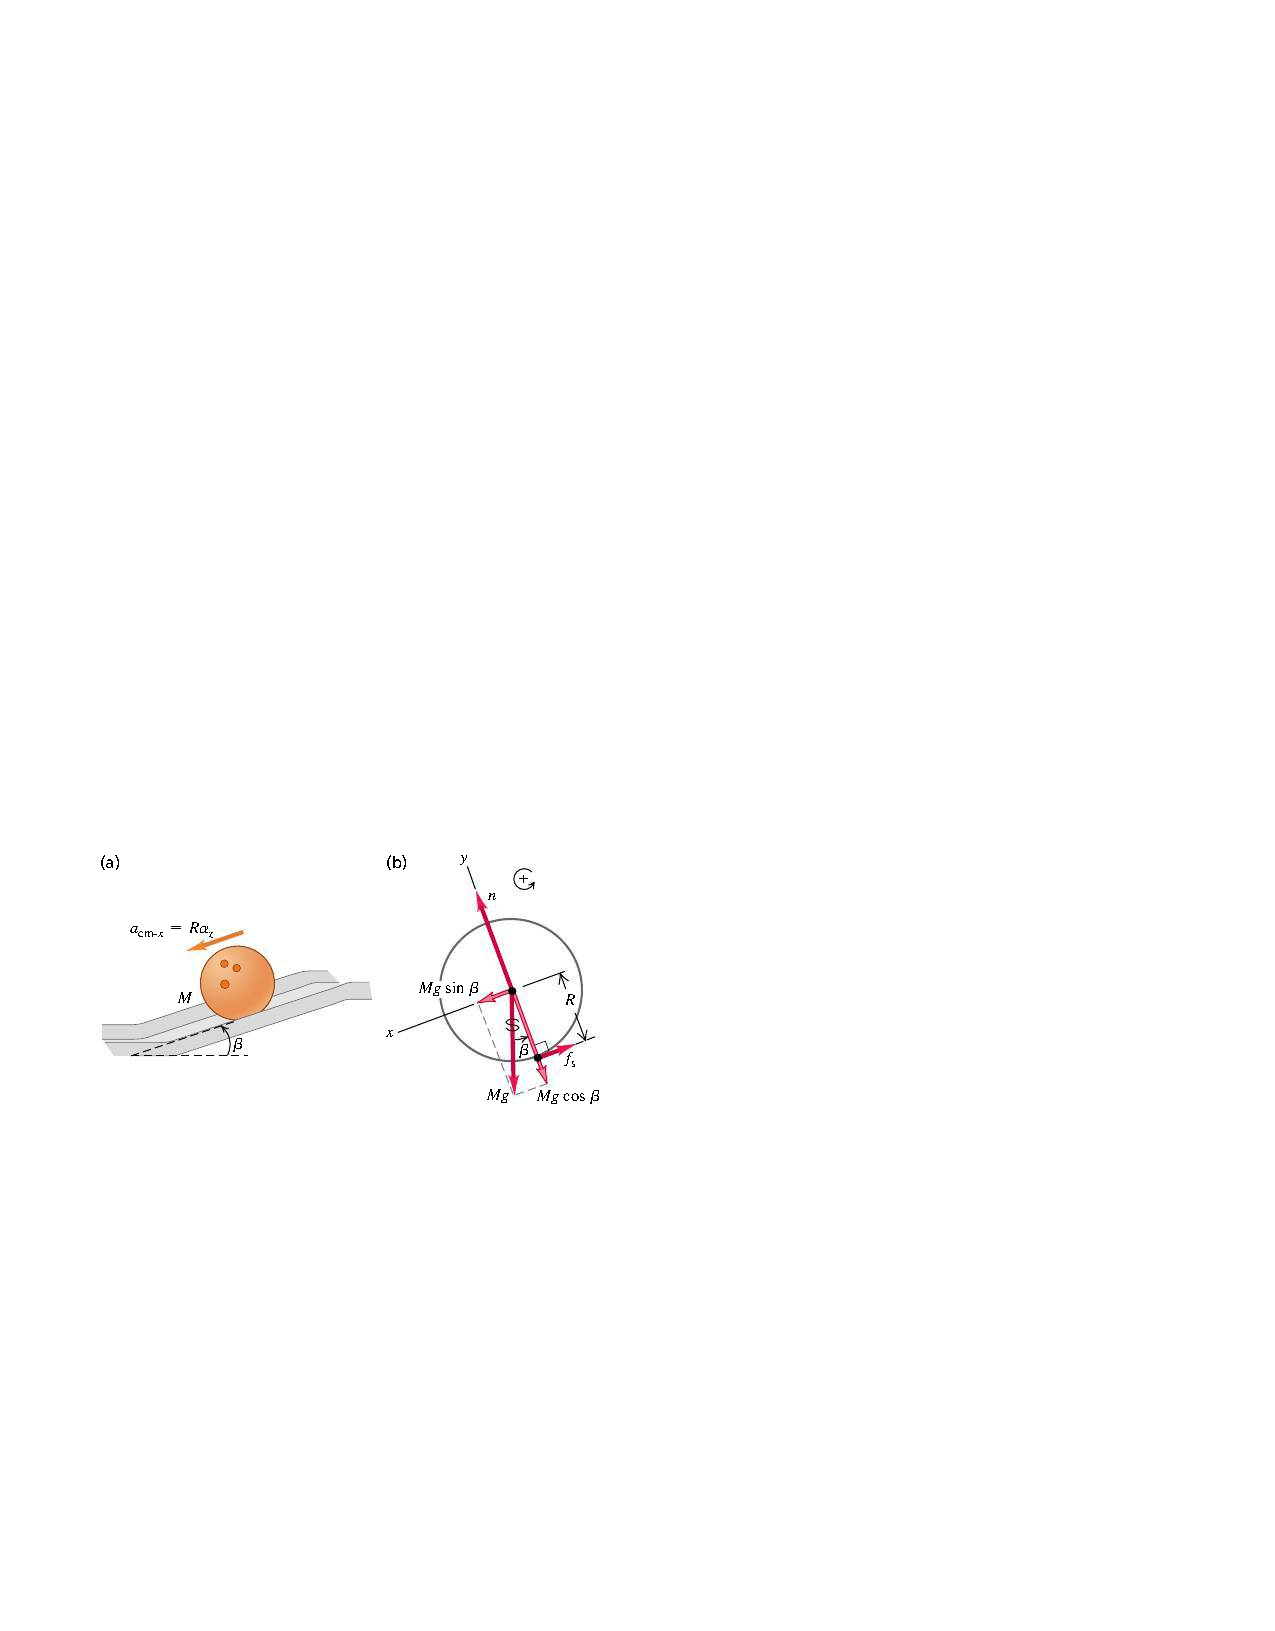
\includegraphics{10-19}
	\caption{\textbf{10.19}}
	\label{10.19}
\end{figure}

\paragraph{Exercise 10.30 (A Ball Rolling Uphill)}
\begin{problem}
	A bowling ball rolls without slipping up a ramp that slopes upward at and angle $\beta$ to the horizontal (see Example 10.7 and Fig.~\ref{10.19}).  Treat the ball as a uniform solid sphere, ignoring the finger holes.
	\begin{enumerate}
		\item Draw the free-body diagram for the ball.  Explain why the friction force must be directed \emph{uphill}.
		\item What is the acceleration of the center of mass of the ball?
		\item What minimum coefficient of static friction is needed to prevent slipping?
	\end{enumerate}
\end{problem}

\begin{solution}
	Example 10.7 describes the same situation, except the ball is rolling downhill.  We can use that worked example to solve this problem.
	
	\begin{enumerate}
		\item The free-body diagram is the same as for Example 10.7, and is shown in Fig.~\ref{10.19}(b).  {\color{blue} The friction force must be directed uphill because it is preventing the ball from \emph{sliding} down the ramp due to gravity.  This is true even when the ball is rolling uphill instead of downhill, because gravity is the only force acting upon the ball, and it always acts downward.}
		\item The free-body diagram is the same as in Example 10.7, so the acceleration of the center of mass is also the same:
			\beq
				a_{\text{cm-}x} = {\color{blue} \frac{5}{7} g \sin{\beta}}.
			\eeq
		Taking note of the $x$ axis as drawn in Fig.~\ref{10.19}(b), we see that the acceleration points \emph{down} the hill.  This means the ball is slowing down as it rolls uphill, which is easily confirmed by physical intuition.
		
		\item We are looking to saturate the inequality
			\beqn \label{stf}
				f \leq \mu_s n,
			\eeqn
			where $f$ is the magnitude of the static friction force, $\mu_s$ is the coefficient of static friction, and $n$ is the magnitude of the normal force acting on the ball.  From Fig.~\ref{10.19}(b),
			\beq
				n = M g \cos{\beta},
			\eeq
		and from Example 10.7,
			\beq
				f = \frac{2}{7} M g \sin{\beta}.
			\eeq
			Now we just need to solve for $\mu_s$ in \refeq{stf}:
			\beq
				\mu_s = \frac{f}{n} = \frac{2}{7} \frac{M g \sin{\beta}}{M g \cos{\beta}} = {\color{blue} \frac{2}{7} \tan{\beta}}.
			\eeq
	\end{enumerate}
\end{solution}


\clearpage
\paragraph{Exercise 10.48 (Asteroid Collision!)}
\begin{problem}
	Suppose that an asteroid traveling straight toward the center of the earth were to collide with our planet at the equator and bury itself just below the surface.  What would have to be the mass of this asteroid, in terms of the earth's mass $M$, for the day to become 25.0\% longer than it presently is as a result of the collision?  Assume that the asteroid is very small compared to the earth and that the earth is uniform throughout.
\end{problem}

\begin{solution}
	We can solve this problem using conservation of angular momentum:
	\beqn \label{consmom}
		I_i \omega_i = I_f \omega_f.
	\eeqn
	When the asteroid hits the earth, its moment of inertia will change from $I_i$ to $I_f$, which will cause its angular velocity to change from $\omega_i$ to $\omega_f$.
	
	According to the problem statement, we can model the earth before the collision as a solid sphere.  This means
	\beq
		I_i = \frac{2}{5} M R^2,
	\eeq
	where $R$ is the radius of the earth.
	
	After the collision, the asteroid is essentially a point mass $m$ stuck to the side of the earth at the equator.  This earth-asteroid system has a center of mass that is some distance $d$ away from the earth's center of mass.  If we fix the origin at the earth's center of mass, then
	\beq
		d = \frac{m R}{m + M}.
	\eeq
	This means the asteroid is orbiting the center of mass with orbital radius $R - d$, so its moment of inertia is
	\beq
		I_a = m (R - d)^2.
	\eeq
	We can use the parallel axis theorem to find the new moment of inertia of the earth:
	\beq
		I_e = I_i + M d^2,
	\eeq
	because $I_i$ is the moment of inertia of the earth rotating about its center of mass.  Finally, the moment of inertia of the entire system is just their sum,
	\beq
		I_f = I_e + I_a = \frac{2}{5} M R^2 + M d^2 + m (R - d) = \frac{2}{5} M R^2 + M \left( \frac{m R}{m + M} \right)^2 + m \left( R - \frac{m R}{m + M} \right)^2.
	\eeq
	
	An earth day is equivalent to the period of the earth's rotation about its axis:
	\beq
		T = \frac{2 \pi}{\omega}.
	\eeq
	For the day to become 25.0\% longer, we need
	\beq
		\frac{T_f}{T_i} = 1.25 \implies \frac{\omega_i}{\omega_f} = 1.25.
	\eeq
	This suggests that we rewrite \refeq{consmom} as
	\beq
		I_f = \frac{\omega_i}{\omega_f} I_i = \frac{5}{4} I_i.
	\eeq
	Feeding our results for the moments of inertia into \refeq{consmom} and solving for the mass of the asteroid, $m$, we find
	\beq
		m = {\color{blue} \frac{M}{9}}.
	\eeq
\end{solution}


\clearpage
\begin{figure} \centering
	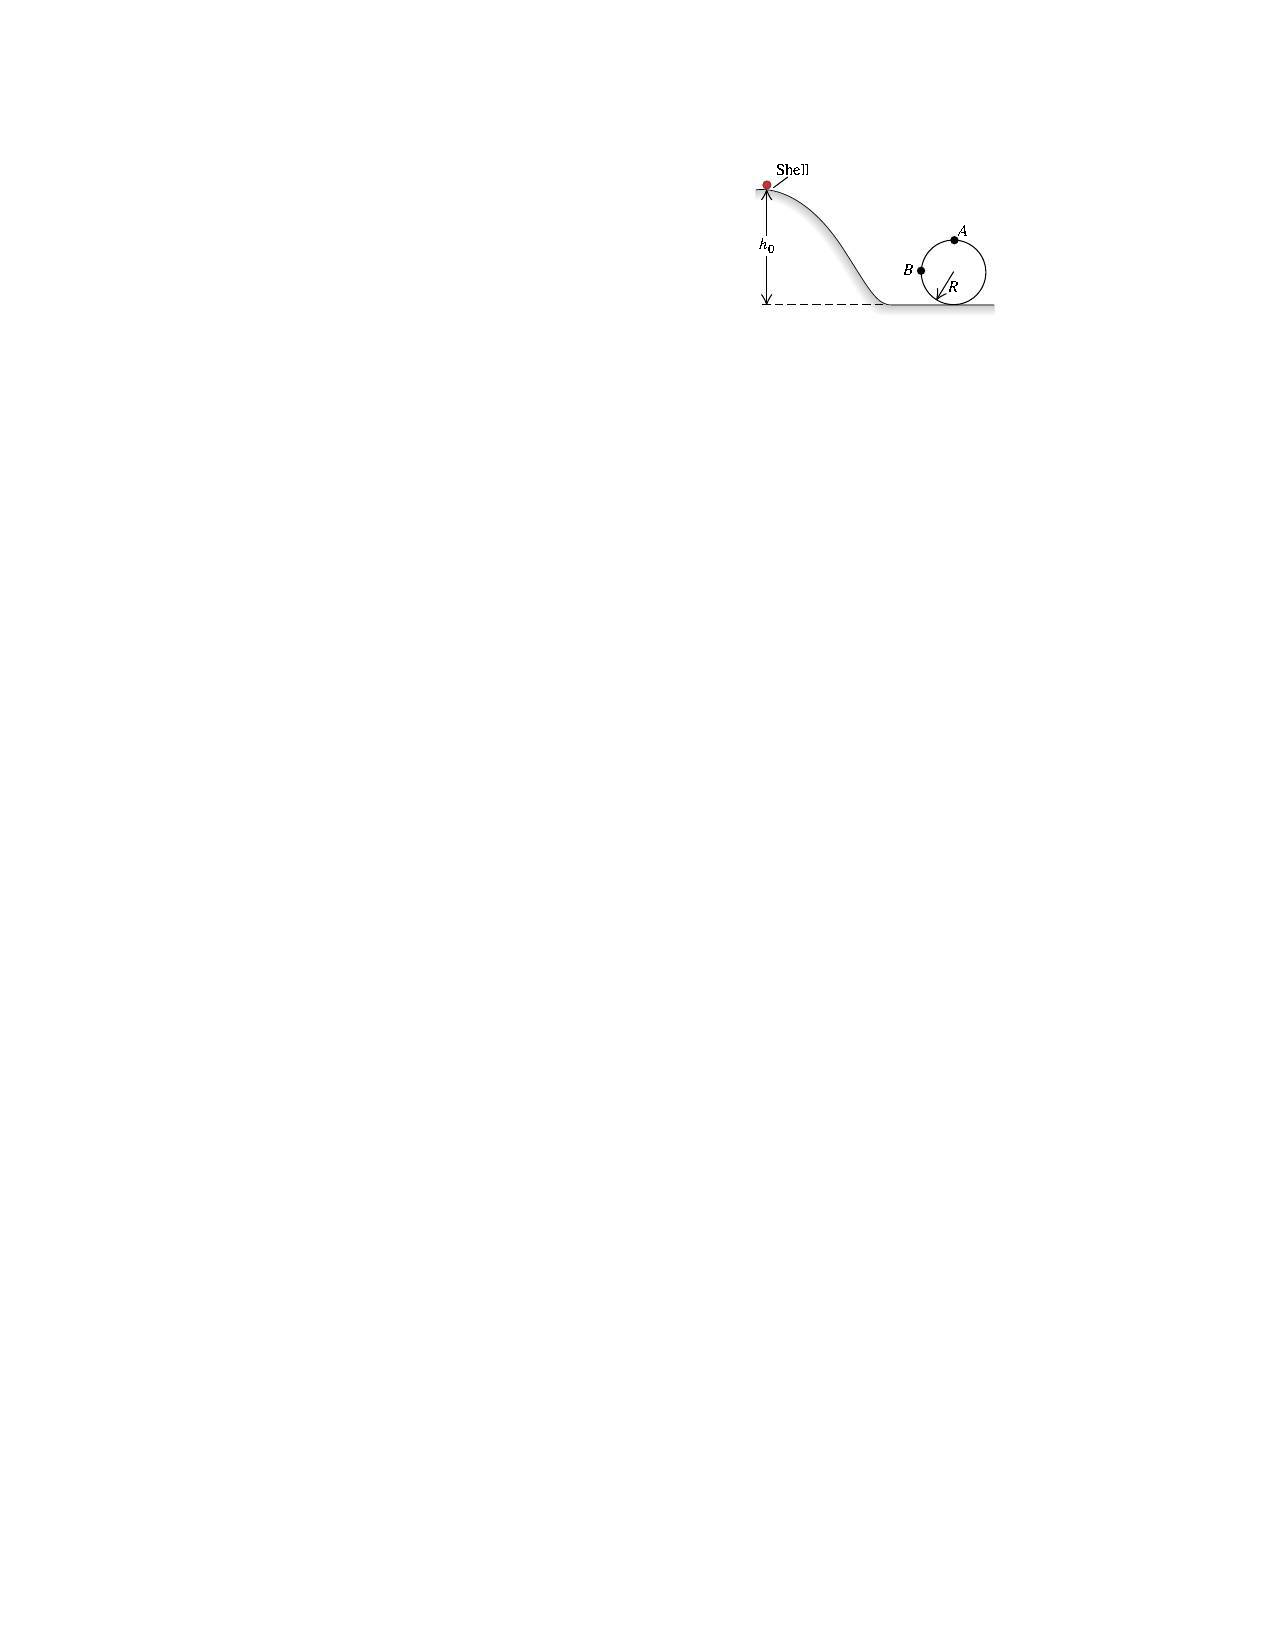
\includegraphics{P10-72}
	\caption{\textbf{P10.72}}
	\label{P10.72}
\end{figure}

\newcommand{\ho}{h_0}

\paragraph{Problem 10.72}
\begin{problem}
	A thin-walled, hollow spherical shell of mass $m$ and radius $r$ starts from rest and rolls without slipping down a track (Fig.~\ref{P10.72}).  Points $A$ and $B$ are on a circular part of the track having radius $R$.  The diameter of the shell is very small compared to $\ho$ and $R$, and the work done by rolling friction is negligible.
	\begin{enumerate}
		\item What is the minimum height $\ho$ for which this shell will make a complete loop-the-loop on the circular part of the track?
		\item How hard does the track push on the shell at point $B$, which is at the same level as the center of the circle?
		\item Suppose that the track had no friction and the shell was released from the same height $\ho$ you found in part (a).  Would it make a complete loop-the-loop?  How do you know?
		\item In part (c), how hard does the track push on the shell at point $A$, the top of the circle?  How hard did it push in part (a)?
	\end{enumerate}
\end{problem}

\begin{solution}
	This is another problem we can solve using conservation of energy.  We are concerned with three states of the system, all of which have the same energy.
	
	Let $U$ be the shell's gravitational potential energy, which is the only potential energy in this system.  When the shell is at points $\ho$, $A$, and $B$, respectively, its potential energy is given by
	\begin{align*}
		U_0 &= m g \ho, \\
		U_A &= 2 m g R, \\
		U_B &= m g R.
	\end{align*}
	For kinetic energy,
	\begin{align}
		K_0 &= 0, \notag \\
		K_A &= \frac{1}{2} m v_A^2 + \frac{1}{2} I \omega_A^2, \label{ka} \\
		K_B &= \frac{1}{2} m v_B^2 + \frac{1}{2} I \omega_B^2, \label{kb}
	\end{align}
	where $v$ is the (translational) speed of the shell, $I$ the moment of inertia about its center of mass, and $\omega$ is its angular speed.
	
	For a spherical shell,
	\beq
		I = \frac{2}{3} m r^2,
	\eeq
	and for rolling without slipping, we have the constraint
	\beq
		\omega = \frac{v}{R}.
	\eeq
	Using these, we can rewrite \refeq{ka} and \refeq{kb}:
	\begin{align}
		K_A &= \frac{1}{2} m v_A^2 + \frac{1}{3} m v_A^2 = \frac{5}{6} m v_A^2, \label{ka2} \\
		K_B &= \frac{5}{6} m v_B^2. \label{kb2}
	\end{align}
	
	\begin{enumerate}
		\item The shell will make a complete loop-the-loop when its speed at point $A$ is great enough to counteract the force of gravity.  The minimum condition is when the centripetal acceleration at $A$ is exactly equal to the gravitational acceleration,
			\beqn \label{centr}
				g = \frac{v_A^2}{R} \implies v_A^2 = g R.
			\eeqn
			This will give us our minimum $\ho$.  Feeding this into \refeq{ka2}, we can invoke conservation of energy between points $\ho$ and $A$:
			\beq
				\Delta K_{0,A} + \Delta U_{0,A} = 0 \implies mg (\ho - 2R) = \frac{5}{6} mg R \implies \ho = {\color{blue} \frac{17}{6} R}.
			\eeq
		
		\item The track will be exerting a normal force $N_B$ on the shell at point $B$, which acts in the horizontal direction.  It is solely responsible for the shell's centripetal acceleration at $B$.  We can find the force by finding the centripetal acceleration, which will look similar to \refeq{centr}.
		
		Invoking conservation of energy between points $\ho$ and $B$, and plugging in our answer for $\ho$, we have
			\beq
				\Delta K_{0,B} + \Delta U_{0,B} = 0 \implies mg (\ho - R) = \frac{5}{6} m v_B^2 \implies \frac{v_B^2}{R} = \frac{11}{5} g.
			\eeq
			Now that we have the centripetal acceleration, we apply Newton's second law to find the force:
			\beq
				N_b = {\color{blue} \frac{11}{5} m g}.
			\eeq
			
		\item If the track has no friction, the shell will have no rotational motion.  So the situation looks just like translational motion problems we have solved before using conservation of energy.  When the shell does not rotate, its kinetic energy at point $A$ is
			\beq
				K_A = \frac{1}{2} m v_A^2.
			\eeq
			The condition for making a complete loop-the-loop is the same, so we need to check whether the shell's velocity still satisfies \refeq{centr} at minimum.  Invoking conservation of energy between points $\ho$ and $A$ using the new $K_A$,
			\beq
				\Delta K_{0,A} + \Delta U_{0,A} = 0 \implies mg (\ho - 2R) = \frac{1}{2} m v_A^2 \implies \frac{v_A^2}{R} = \frac{5}{3} g.
			\eeq
			{\color{blue} Yes, the shell will make a complete loop-the-loop, because its speed in this case is \emph{greater} than what is required to counteract the force of gravity at point $A$.}
			
		\item As we did in (b) for point $B$, we can calculate the normal force exerted by the track at point $A$.
			
			In part (c), we know that the centripetal acceleration at $A$ is greater than $g$, so the normal force is contributing to the centripetal force $F_c$:
			\beq
				F_c = N_A + m g \implies N_A = \frac{5}{3} m g - m g = {\color{blue} \frac{2}{3} m g}.
			\eeq
			In part (a), the condition we enforced to find the minimum $\ho$ was that the centripetal acceleration at $A$ was \emph{exactly} equal to $g$, so there can be no forces acting upon the shell other than gravity.  In other words,
			\beq
				N_A = {\color{blue} 0}.
			\eeq
	\end{enumerate}
\end{solution}


\clearpage
\begin{figure}[b]
	\vspace{1.5in}
	\caption{Free-body diagram for 10.76.}
	\label{P10.76}
\end{figure}

\paragraph{Problem 10.76}
\begin{problem}
	You are designing a system for moving aluminum cylinders from the ground to a loading dock.  You use a sturdy wooden ramp that is \SI{6.00}{\meter} long and inclined at $37.0^\circ$ above the horizontal.  Each cylinder is fitted with a light, frictionless yoke through its center, and a light (but strong) rope is attached to the yoke.  Each cylinder is uniform and has mass \SI{460}{\kg} and radius \SI{0.300}{\meter}.  The cylinders are pulled up the ramp by applying a constant force $\vF$ to the free end of the rope.  $\vF$ is parallel to the surface of the ramp and exerts no torque on the cylinder.  The coefficient of static friction between the ramp surface and the cylinder is 0.120.
	\begin{enumerate}
		\item What is the largest magnitude $\vF$ can have so that the cylinder still rolls without slipping as it moves up the ramp?
		\item If the cylinder starts from rest at the bottom of the ramp and rolls without slipping as it moves up the ramp, what is the shortest time it can take the cylinder to reach the top of the ramp?
	\end{enumerate}
\end{problem}

\begin{solution}
	This problem is a lot like \textbf{10.30}, but with the addition of an external force acting upon the cylinder which pulls it uphill.  Here the net force is directed \emph{uphill}, and therefore the cylinder's translational acceleration points uphill.  This reverses the direction of the static friction force with respect to what we saw in \textbf{10.30}.  A free-body diagram for one of the cylinders is shown in Fig.~\ref{P10.76}, which may be compared to Fig.~\ref{10.19}(b).
	
	Using Newton's second law, we can use Fig.~\ref{P10.76} to write two equations: one for translational motion, and one for rotational motion.  Let $f$ be the magnitude of the static friction force, $m$ the mass of the cylinder, and $\theta$ the inclination of the ramp.  For translational motion,
	\beqn \label{trans}
		F = f + m g \sin{\theta} \implies ma = F - f - m g \sin{\theta},
	\eeqn
	where $a$ is the cylinder's translational acceleration.
	
	Let $r$ be the radius of the cylinder.  For rotational motion, only $f$ exerts a torque on the cylinder, which has lever arm $r$.  This means
	\beqn \label{rot0}
		f r = I \alpha,
	\eeqn
	where $\alpha$ is the cylinder's rotational acceleration, and the moment of inertia
	\beq
		I = \frac{1}{2} m r^2
	\eeq
	for a cylinder, so \refeq{rot0} becomes
	\beqn \label{rot}
		f = \frac{1}{2} m r \alpha.
	\eeqn
	
	From \refeq{trans}, $F$ will have its largest magnitude when $f$ is maximized.  In general, the static friction force is given by
			\beqn \label{stat}
				f \leq \mu_s N = \mu_s m g \cos \theta,
			\eeqn
			where $\mu_s$ is the coefficient of static friction, and the normal force $N$ is shown in Fig.~\ref{P10.76}.  We need to saturate this equality in order to find the largest possible $F$.
		
	Rolling without slipping imposes the constraint
	\beq
		\alpha = \frac{a}{r},
	\eeq
	which changes \refeq{rot} to
	\beq
		f = \frac{1}{2} m a.
	\eeq
	Equating this with \refeq{stat} gives us
	\beqn \label{fric}
		\frac{1}{2} m a = \mu_s m g \cos \theta.
	\eeqn
	We can also use it to rewrite \refeq{trans} as
	\beqn \label{frac}
			ma = F - \frac{1}{2} m a - m g \sin{\theta}.
	\eeqn
	Now we have the system of two equations \refeq{fric} and \refeq{frac} with two unknowns, $F$ and $a$.  The solutions are
	\begin{align}
		a &= 2 \mu_s g \cos{\theta}, \label{acyl} \\
		F &= 3 \mu_s m g \cos{\theta} + m g \sin{\theta}. \label{Fcyl}
	\end{align}
			
	\begin{enumerate}
		\item Plugging numbers into \refeq{Fcyl},
			\beq
				F = 3 (0.120) (\SI{460}{\kg}) (\sig) \cos{37.0^\circ} + (\SI{460}{\kg}) (\sig) \sin{37.0^\circ} = {\color{blue} \SI{4010}{\newton}}.
			\eeq
			
		\item We know from (a) that the maximum possible acceleration up the ramp is given by \refeq{acyl}.  This is a constant acceleration in the $x$ direction, and the cylinder needs to travel the entire length $\ell$ of the ramp, as shown in Fig.~\ref{P10.76c}.
		
			We can use one-dimensional kinematics to describe the translation of the cylinder's center of mass.  Since the cylinder starts from rest,
			\beqn \label{time}
				\ell = \frac{1}{2} a t^2 \implies t = \sqrt{\frac{2 \ell}{a}}.
			\eeqn
			Plugging numbers into \refeq{acyl},
			\beq
				a = 2 (0.120) (\sig) \cos{37.0^\circ} = \SI{1.88}{\meter\per\square\second}.
			\eeq
			Finally, plugging numbers into \refeq{time},
			\beq
				t = \sqrt{\frac{2 (\SI{6.00}{\meter})}{\SI{865}{\meter\per\square\second}}} = {\color{blue} \SI{2.53}{\second}}.
			\eeq
	\end{enumerate}
\end{solution}

\begin{figure}[b]
	\caption{Schematic diagram for 10.76.}
	\label{P10.76c}
\end{figure}


\clearpage
\begin{figure} \centering
	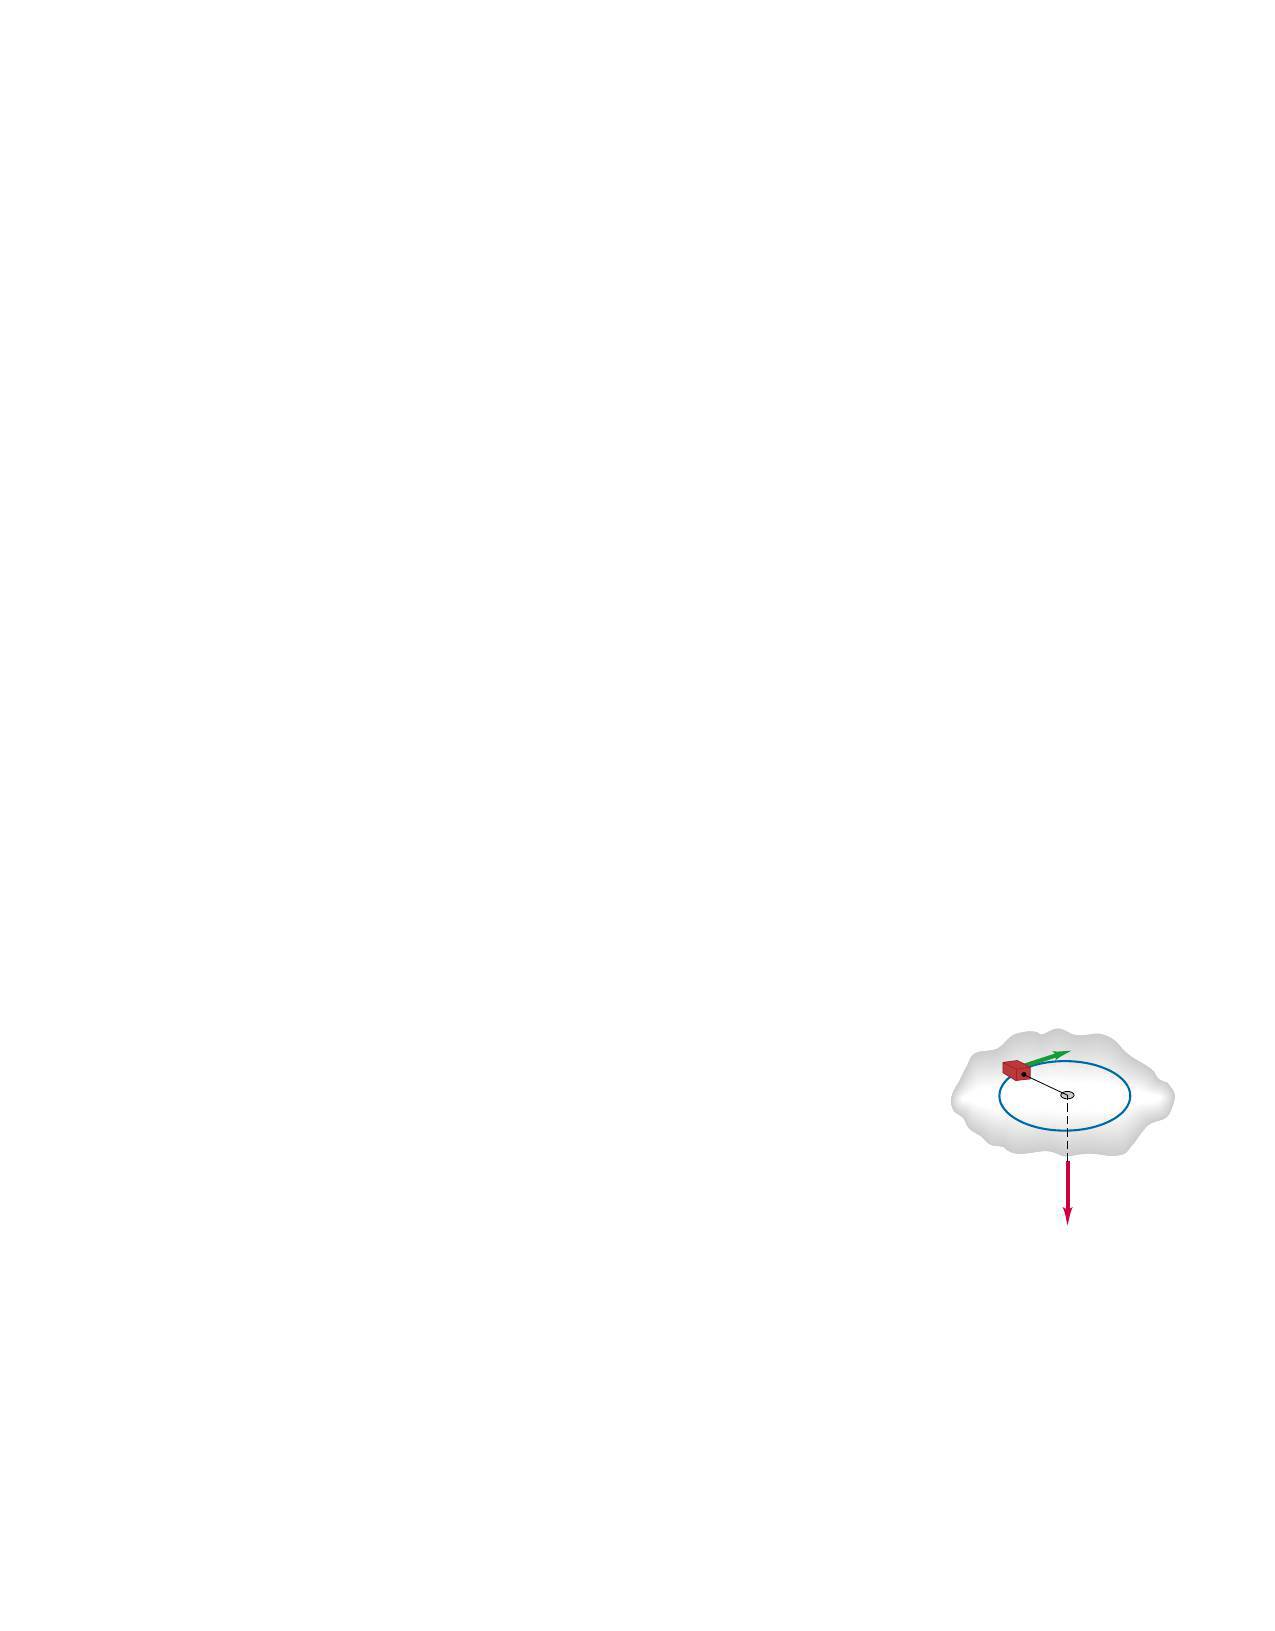
\includegraphics{E10-42}
	\caption{\textbf{E10.42}}
	\label{E10.42}
\end{figure}

\paragraph{Problem 10.86}
\begin{problem}
	A small block with mass \SI{0.130}{\kg} is attached to a string passing through a hole in a frictionless, horizontal surface (see Fig.~\ref{E10.42}).  The block is originally revolving in a circle with a radius of \SI{0.800}{\meter} about the hole with a tangential speed of \SI{4.00}{\meter\per\second}.  The string is then pulled slowly from below, shortening the radius of the circle in which the block revolves.  The breaking strength of the string is \SI{30.0}{\newton}.  What is the radius of the circle when the string breaks?
\end{problem}

\begin{solution}
	This is another problem about conservation of angular momentum.  Since the block is small, we can treat it as a point mass.  For a point mass,
	\beq
		I = m R^2,
	\eeq
	where $m$ is the block's mass and $R$ its orbital radius.
	
	We are given the block's initial orbital radius $R_i$ and its initial tangential speed $v_i$.  Its initial angular velocity is then
	\beq
		\omega_i = \frac{v_i}{R_i}.
	\eeq
	We can write the block's initial angular momentum in terms of known quantities:
	\beqn \label{momi}
		I_i \omega_i = m v_i R_i.
	\eeqn
	The final state of the system is the instant at which the string breaks.  Call its breaking force $T$.  Since the block is moving in a circle,
	\beqn \label{brforce}
		T = \frac{m v_f^2}{R_f}.
	\eeqn
	We can divide both sides of \refeq{brforce} by $R_f$ to get an expression for the final angular velocity:
	\beq
		\frac{T}{R_f} = m \frac{v_f^2}{R_f^2} = m \omega_f^2 \implies \omega_f = \sqrt{\frac{T}{m R_f}}.
	\eeq
	Now we can write the final angular momentum in terms of known quantities and $R_f$:
	\beqn \label{momf}
		I_f \omega_f = m R_f^2 \sqrt{\frac{T}{m R_f}} = \sqrt{m R_f^3 T}.
	\eeqn
	Finally, we can equate \refeq{momi} and \refeq{momf} and solve for $R_f$:
	\beq
		m v_i R_i = \sqrt{m R_f^3 T} \implies R_f = \left( \frac{m R_i^2 v_i^2}{T} \right)^{1/3}.
	\eeq
	Plugging in numbers,
	\beq
		R_f = \left( \frac{(\SI{0.130}{\kg}) (\SI{0.800}{\meter})^2 (\SI{4.00}{\meter\per\second})^2}{\SI{30.0}{\newton}} \right)^{1/3} = {\color{blue} \SI{0.354}{\meter}}.
	\eeq
\end{solution}

\end{document}